% Copyright (C)  2016  Orestis Malaspinas.
%     Permission is granted to copy, distribute and/or modify this document
%     under the terms of the GNU Free Documentation License, Version 1.3
%     or any later version published by the Free Software Foundation;
%     with no Invariant Sections, no Front-Cover Texts, and no Back-Cover Texts.
%     A copy of the license can be downloaded from:
%     https://www.gnu.org/licenses/fdl.html.

\documentclass[a4paper,12pt]{book}
\usepackage[utf8]{inputenc}
\usepackage[french]{babel}
\usepackage{amsfonts,bm,amsmath,amssymb,graphicx,amsthm}
\usepackage{cancel}
\usepackage{mathtools}
\usepackage{caption}
\usepackage{hyperref}

\setlength{\parindent}{0pt}

\newcommand{\real}{\mathbb{R}}
\newcommand{\integer}{\mathbb{Z}}
\renewcommand{\natural}{\mathbb{N}}
\newcommand{\complex}{\mathbb{C}}
\newcommand{\zbar}{\bar{z}}
\newcommand{\dd}{\mathrm{d}}
\newcommand{\perm}{\mathrm{perm}}
\newcommand{\card}{\mathrm{card}}
\newcommand{\fh}{\hat{f}}
\newcommand{\gh}{\hat{g}}
\newcommand{\hh}{\hat{h}}
\renewcommand{\Re}{\mathrm{Re}}
\renewcommand{\Im}{\mathrm{Im}}
\newcommand{\pDeriv}[2]{\frac{\partial #1}{\partial #2}}
\newcommand{\pDerivTwo}[2]{\frac{\partial^2 #1}{\partial #2^2}}
\newcommand{\dDeriv}[2]{\frac{\dd #1}{\dd #2}}
\newcommand{\dDerivTwo}[2]{\frac{\dd^2 #1}{\dd #2^2}}
\newtheorem{definition}{Définition}
\newtheorem*{exemples}{Exemples}
\newtheorem*{exemple}{Exemple}
\newtheorem{exercice}{Exercice}
\newtheorem*{exercices}{Exercices}
\newtheorem*{remarque}{Remarque}
\newtheorem{proprietes}{Propriétés}
\newtheorem{theoreme}{Théorème}
\newcommand{\cm}{\mathrm{cm}}
\newcommand{\km}{\mathrm{km}}
\newcommand{\mm}{\mathrm{mm}}
\newcommand{\cd}{\mathrm{cd}}
\newcommand{\mol}{\mathrm{mol}}
\newcommand{\m}{\mathrm{m}}
\newcommand{\s}{\mathrm{s}}
\newcommand{\kg}{\mathrm{kg}}
\newcommand{\K}{\mathrm{K}}
\newcommand{\C}{\mathrm{C}}
\newcommand{\A}{\mathrm{A}}
\newcommand{\N}{\mathrm{N}}
\newcommand{\V}{\mathrm{V}}
\newcommand{\W}{\mathrm{W}}


\title{Résumé du cours de Physique Générale}
\author{Orestis Malaspinas}

\begin{document}
\maketitle

\chapter{Mesures, incertitudes, et estimations}

Pour celles et ceux qui sont intéressés par plus de détails, vous pouvez vous référer au cours de métrologie de l'EPFL par exemple: \url{http://sb.epfl.ch/page-52191-en.html}

\section{Généralités}

Toues les sciences ``naturelles'' sont basées sur \textit{l'observation} du monde qui nous entoure. 
Mais malgré le fait qu'on ait l'impression que le processus d'osbervation soit une suite simple:
observation, expérimentation, obtention de résultats, qu'on explique avec une \textit{théorie} (un ensemble de \textit{lois}) cela n'est pas vraiment le cas. En fait,
de façon proche à ce qui se passe dans les arts, les sciences sont un processus hautement créatif. 
En effet, lors d'une observation un scientifique ne décrit pas tout ce qu'il voit, 
mais sélectionne uniquement ce qu'il juge important
pour la compréhension et l'interprétation d'un phénomène. De plus, une fois sélectionné
le processus à observer, il convient de créer une expérience permettant de le mesurer de façon aussi précise que possible
pour pouvoir le décrire. La mesure tient donc une place centrale dans les sciences et se complète parfaitement avec la création de théories
qui permettent l'explication d'observations. Par ailleurs, toutes les théories ne sont pas le fruit
d'expériences (ou d'observations) mais ont souvent été le résultat de constructions de l'esprit. 
Dans ce cas les expériences, viennent confirmer (ou infirmer) les théories. En effet, une théorie physique est
supposée vraie jusqu'à ce qu'une expérience vienne l'infirmer (on ne peut pas prouver une théorie).

Les expériences ont donc deux fonctions principales
\begin{itemize}
 \item Collecter des données qui permettront la dérivation de lois physiques.
 \item Vérifier ou infirmer les lois physiques.
\end{itemize}

Les lois physiques sont des outils très pratiques permettant la prédiction \textit{quantitative} 
de phénomènes (et non la ``post-diction'' comme avec les expériences). Il est par exemple possible de prédire très précisément la hauteur à laquelle il faut lancer un satellite 
pour qu'il se retrouve en orbite géostationnaire (et donc connâitre la quantité de carburant nécessaire par exemple) grâce aux lois de Newton. 
Ce qui serait certainement beaucoup plus difficile à déterminer expérimentalement, s'il fallait faire des dizaines d'essais jusqu'à ce que ça marche.

Par ailleurs, beaucoup de ``lois'' ont des capacités prédictives mais ne sont pas complètement générales. Par exemple, bien que les lois de Newton 
marchent très très bien pour notre vie de tous les jours, certaines applications d'usage quotidien ne fonctionneraient pas si on s'en tenait là. 
En effet, le GPS requiert l'extension des lois de Newton à la relativité générale pour pouvoir fonctionner correctement. En fait
la gravitation Newtonienne est une approximation de la relativité générale.

Ces approximations sont souvent le résultat de simplifications faites dans la représentation dont ont se fait 
de processus physiques: les \textit{modèles}. Un modèle est une vision de l'esprit qui permet de réunir plusieurs
situations qui à première vue peuvent paraître non-semblables ou à simplifier un problème afin de pouvoir le résoudre plus simplement. 
Par exemple un liquide est composé d'atomes qui se déplacent. Il serait possible (mais complètement infaisable et inutile dans presque tous les cas) 
d'étudier chaque atome indviduellement pour avoir une descfription très détaillée du mouvement d'un fluide. Néamoins, il est beaucoup plus simple de 
faire \textit{l'hypothèse} qu'un fluide peut être considéré comme un objet continu.

\section{Mesure et incertitude}

Comme nous venons de le dire les mesures tiennent une place primordiale en physique. Mais toute mesure ne peut être 
parfaite et contient donc une part d'incertitude. En générale l'incertitude d'une mesure provient 
de la précision limitée des instruments utilisés. Par exemple, lors de la mesure d'une longueur avec une règle,
la graduation est en générale faite à chaque millimètre. Il est donc impossible d'être plus précis
que le millimètre (on pourrait éventuellement dire qu'on est précis à 0.5 millimètres, mais il faudrait pour cela que l'utilisateur de la 
règle ait de très très très bons yeux, que le fabriquant de la règle ait un processus absolument parfait de graduation, etc).
Si la longueur, $L$, d'un objet mesuré à la règle est de $10.1\cm$, on peut donner l'information de l'incertitude 
en ajoutant derrière le sigle $\pm 0.1\cm$ ou
\begin{equation*}
 L=10.1\pm0.1\ \cm.
\end{equation*}
Cela signifie que la valeur de $L$ est située quelque part entre $10$ et $10.2$ centimètres.
Une autre façon de mesurer la précision d'une mesure est de donner l'erreur en pourcentage de la mesure effectuée.
Ici nous aurions que l'erreur est de
\begin{equation*}
 \frac{0.1}{10.1}\cdot 100\cong 1\%.
\end{equation*}
Cette façon de quantifier l'erreur dépend donc de la valeur de la quantité mesurée (plus la longueur mesurée est grande plus
le pourcentage sera petit et inversément).


Une autre source d'incertitude peut provenir de la nature du phénomène observé. Si nous mesurions aujourd'hui la température 
à un endroit donné de Genève durant toute la journée nous verrions une cretaine courbe de température. Cette courbe serait certainement
différente de la courbe du lendemain ou de celle du même jour de l'année d'après. Ces mesures non reproductibles 
doivent donc faire l'objet d'études statistiques et contiennent des incertitudes de nature très différentes (en plus des erreurs dûes aux mesures
elles-mêmes).

\subsection{Chiffres significatifs}

Le nombre de chiffres significatifs est le nombre de chiffres d'un résultat dont la valeur est ``sûre''. Le nombre $1.23$ contient trois chiffres 
significatifs tout comme le nombre $0.0123$ (les zéros ne sont là que pour placer la virgule). La façon dont on donne un résultat
permet donc d'indiquer avec quelle précision nous connaissons un résultat. Il est souvent tentant d'exprimer un résultat avec un grand nombre de chiffres
significatifs, mais cela peut s'avérer extrêmement contre productif car cela donne une fausse impression de grande précision d'une mesure.
Si nous reprenons notre mesure avec la règle de la longueur $L=10.1$. En se donnant un peu de peine on peut facilement se convaincre qu'on a
pas exactement $10.1$ mais un peu plus disons $10.15$. Même si cela n'est pas vraiment grave dans ce cas, le $5$ est totalement superflu
car il est complètement impossible de dire si cela est 10.15 ou 10.13 ``à l'oeil''. De façon générale si notre précision avait été de $\pm 1\cm$
on aurait écrit $L=10$, à $\pm 0.1$ on écrit $10.1$, à $\pm 0.01$ on écrit $10.10$, etc. Par ailleurs, lonrsqu'on combine des valeurs contenant
des incertitudes il faut également faire attention. Supposons que nous ayons un carré dont le coté fait $10.1\cm$, sa surface est de 
$10.1^2=102.01$. Hors, la valeur de la surface est incluse entre les deux valeurs extrêmes possibles: $10^2=100$ et $10.2^2=104.04$. Il est 
donc inutile de garder $0.01$ et on donne la valeur de $102$ pour la surface.

Il est commun d'écrire les nombre en \textit{notation scientifique} ou en puissances de $10$. Le nombre $10'100$ s'écrit $1.01\cdot 10^4$ en notation
scientifique, le nombre $0.001234=1.234\cdot 10^{-3}$, ... Un des avantages de la notation scientifique, c'est qu'elle permet immédiatement de connaître le nombre de chiffres
significatifs d'un résultat: il correspnd au nombre de chiffres composant le nombre multiplié par la puissance de $10$.

\section{Unités, Système International}

Toute mesure doit être effectuée par rapport à un ``standard'' ou unités. Cela n'a aucun sens de dire qu'un éléphant pèse 36, si nous ne disons pas
36 en quelles unités. Pour chaque grandeur de multiple standards ont été créé au cours des années qui sont devenus de plus en plus précis
avec les avancées technologiques (combien exactement mesure 1m, la durée d'une seconde, etc). 
Dans cette section nous allon discuter les unités des grandeurs de base  de la physique. Nous verrons en particulier le \textit{Système International} (ou SI).

Les unités sont définies par rapport à des grandeurs ``facilement'' mesurables avec une grade précision et qui ne changent pas (ou très très très peu)
au cours du temps.

\subsection{Longueur}

Le standard international fût établi par la France dans les années 1790. 
Pour les unités de longueur est le mètre (abregé $\m$). A l'origine le mètre était 1/10'000'000 de la distance entre l'équateur et un des pôles.
A partir de cette mesure un étalon en platine fût forgé (c'est quand même plus pratique à utiliser). Puis, en 1889, le mètre a été défini comme la distance entre deux très fines encoche sur une barre d'un alliage platine-irridium. Comme cette façon de définir le mètre n'était pas suffisamment précise pour beaucoup d'applications, en 1960
le mètre devint $1'650'763.73$ longueur d'onde d'une lumière émise par le gaz krypton-86. En 1983, fût redéfini comme la distance parcourue par la lumière en 1/299'792'458 secondes.

Il existe d'autres unités de longueur, par exemple les britaniques utilisent le pouce  ou inch (1$\mathrm{in.}$ correspond à 0.0254$\m$). Dans ce cours nous nous concentrerons principalement
sur le système SI.

\subsection{Temps}

La mesure du temps en SI est donnée en secondes (abrégée $\s$). Une seconde a longtemps été définie comme étant $1/(3600\cdot 24)=1/86'000$-ème
de journée solaire. La vitesse de rotation de la terre se ralentissant légérement d'année en année, il a été nécessaire de raffiner de plus en plus 
cette définition. A présent une seconde correspond à un processus atomique. Il s'agit du temps nécessaire à 9'192'631'770 de 
la transitions entre deux états de l'atome de césium 133. 

\subsection{Masse}

Le kilogramme (abrégé $\kg$) est la masse d'un étalon international du kilogramme. En 1795, le kilogramme était la d'un décimètre cube 
d'eau à une température de $4^\circ\C$. Puis il a été remplacé par un étalon en platine irridé (voir Fig.~\ref{fig_kg}). Il s'agit de la seule unité utilisant encore un étalon, 
aucune ``grandeur naturelle'' n'ayant pu être utilisée pour définir le kilogramme autrement. Des copies de cet étalon ont été fabriquée et envoyées à
chaque état qui en ont fait d'autres copies officielles pour contrôler les balances utilisées un peu partout sur les territoires.
\begin{figure}
\begin{center}
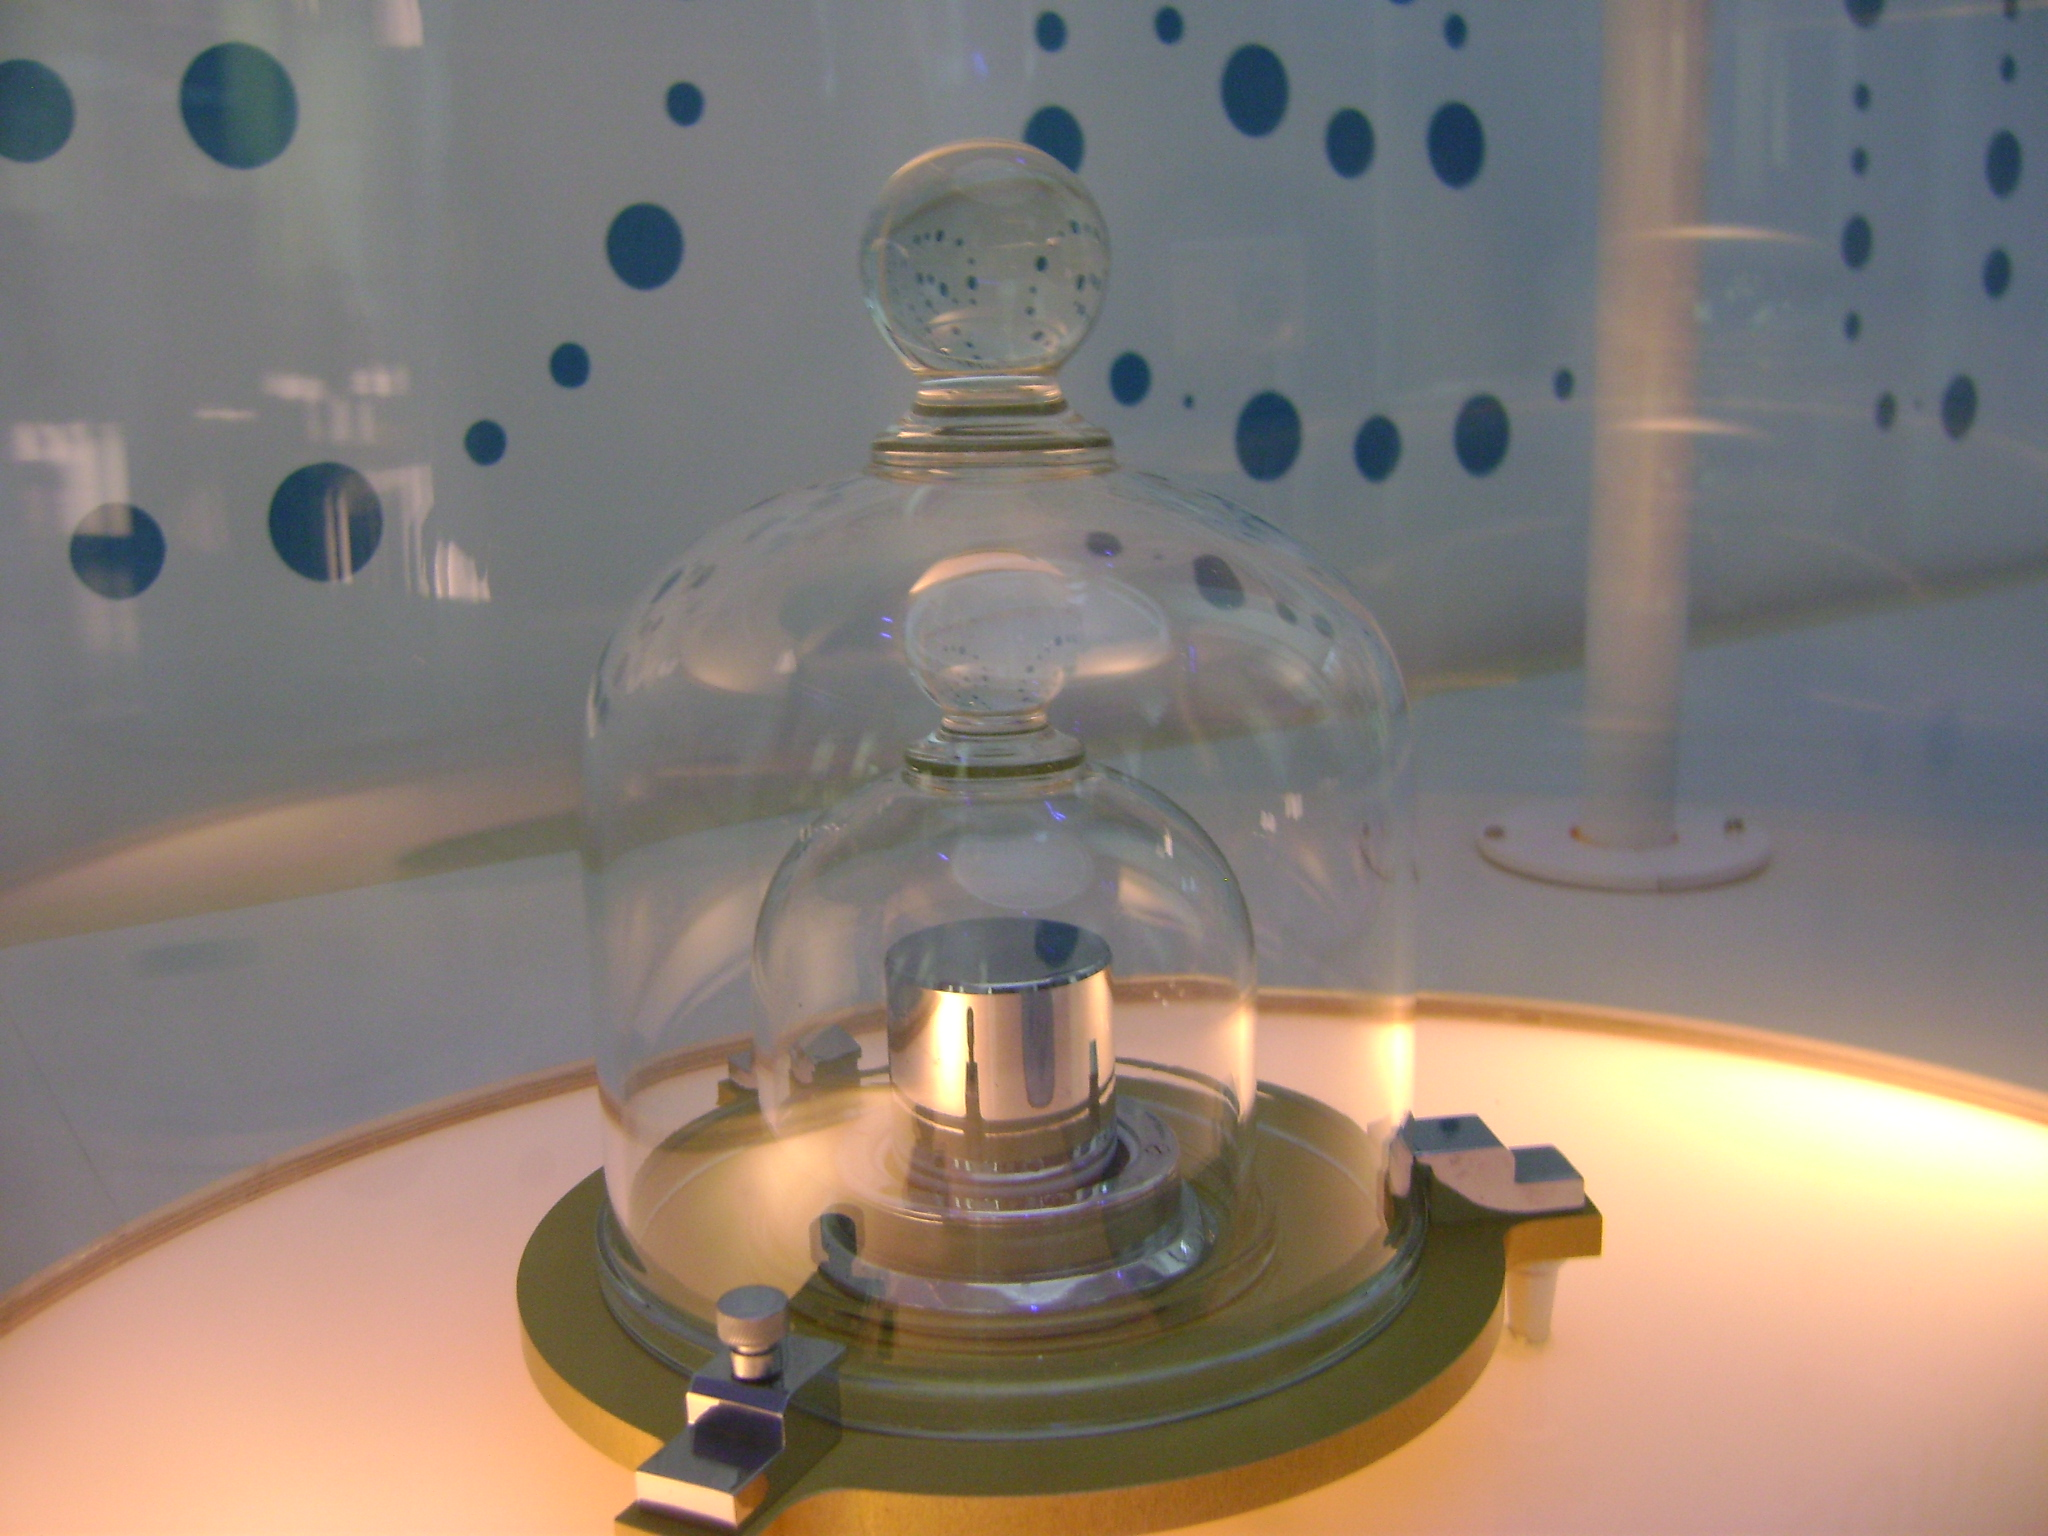
\includegraphics[width=0.5\textwidth]{figs/kilogram_replica.jpg}
\caption{Une réplique de l'étalon international du kilogramme présentée à la cité des sciences et de l'industrie (Vilette), source: \url{https://upload.wikimedia.org/wikipedia/commons/a/ac/Prototype_kilogram_replica.JPG}}
\label{fig_kg}
\end{center}
\end{figure}

\subsection{Température}

La température mesure le degré d'échauffement d'un corps. En SI l'unité de la température est le degré Kelvin (abrégé $\K$).
Il est défini comme le $1/273.16$-ème de la température du point triple de l'eau (la température où les trois phases, solides, liquides, gazeuse, de l'eau 
peuvent coexister en équilibre thermodynamique). Cette température se trouve par définition à $273.16^\circ\K$ ou encore à $0.01^\circ\C$.
Nous verrons un peu plus de détails sur la définition du zéro degrés Kelvin (ou zéro absolu) dans la suite du cours.

\subsection{Courant}

L'intensité du courant électrique est mesurée en Ampères (abrégé $\A$). Un ampère est l'intensité de courant constant qui circulerait 
dans deux fils conducteurs infinis placés dans le vide, de section négligeable, et placés à une distance d'un mètre l'un de l'autre 
qui produirait une force de $2\cdot 10^{-7}$ Newton par longueur de mètre. Les autres unités très utiles en électicité, l'ohm (abrégé $\Omega$) et 
le volt (abrégé $\V$) se déduisent ensuite par les fameuse formules $U=R\cdot I$ ($[\V]=[\Omega]\cdot [\A]$) et $P=U\cdot I$ ($[\W]=[\V]\cdot [\A]$).

\subsection{Quantité de matière}

La quantité de matière se mesure en moles (abrégé $\mol$). Une mole de matière contient autant de particules que 
$0.012\kg$ contient d'atomes de Carbone 12 soit environ $6.02\cdot 10^{23}$ atomes (on appelle ce nombre, le nombre d'Avogadro ou de Loschmidt). 
Cette valeur est étonnament constante. Pour
tout élément du tableau périodique une mole sera le nombre d'atomes d'élément de poids atomique $N$, dans $N$ grammes de matière.

\subsection{Intensité lumineuse}

L'intensité lunineuse est mesurée en candela (abrégé $\cd$). Elle est donnée par l'intensité lumineuse émise par
une source monochromatique de fréquence de $540\cdot 10^{12}\s^{-1}$ et dont l'intensité énergétique est de 
$1/683 \W$ par stéradian (équivalent du radian mais sur une sphère).

\subsection{Préfixes du Système International}

Pour exprimer les puissances de 10 du SI, un certain nombre de préfixes ont été définis pour simplifier 
les notations (voir la Table~\ref{table_prefixe}). Il est relativement aisé de convertir entre les différents préfixes.
Ainsi $23\cm$ correspondent à $230\mm$ ou $0.23\m$. Pour le calcul de surfaces (ou d'unités prises à une certaine puissance les choses
se compliquent un tout petit peu. Ainsi le préfixe est complètement attaché à l'unité. Par exemple les unités d'un volume
se convertissent comme
\begin{equation}
 23\cm^3=23\cdot(10^{-2} m)^3=23\cdot 10^{-6}m^3.
\end{equation}

\begin{table}
\begin{tabular}{|l|l|l|l|l|}
\hline
$10^n$&Préfixe français&Symbole&Nombre décimal&Désignation\\
\hline\hline
$10^{24}$&yotta&Y&1 000 000 000 000 000 000 000 000&Quadrillion\\
\hline
$10^{21}$&zetta&Z&1 000 000 000 000 000 000 000&Trilliard\\
\hline
$10^{18}$&exa&E&1 000 000 000 000 000 000&Trillion\\
\hline
$10^{15}$&péta&P&1 000 000 000 000 000&Billiard\\
\hline
$10^{12}$&téra&T&1 000 000 000 000&Billion\\
\hline
$10^{9}$&giga&G&1 000 000 000&Milliard\\
\hline
$10^{6}$&méga&M&1 000 000&Million\\
\hline
$10^{3}$&kilo&k&1 000&Millier\\
\hline
$10^{2}$&hecto&h&100&Centaine\\
\hline
$10^{1}$&déca&da&10&Dizaine\\
\hline
$10^{0}$&(aucun)&—&1&Unité\\
\hline
$10^{-1}$&déci&d&0,1&Dixième\\
\hline
$10^{-2}$&centi&c&0,01&Centième\\
\hline
$10^{-3}$&milli&m&0,001&Millième\\
\hline
$10^{-6}$&micro&$\mu$&0,000 001&Millionième\\
\hline
$10^{-9}$&nano&n&0,000 000 001&Milliardième\\
\hline
$10^{-12}$&pico&p&0,000 000 000 001&Billionième\\
\hline
$10^{-15}$&femto&f&0,000 000 000 000 001&Billiardième\\
\hline
$10^{-18}$&atto&a&0,000 000 000 000 000 001&Trillionième\\
\hline
$10^{-21}$&zepto&z&0,000 000 000 000 000 000 001&Trilliardième\\
\hline
$10^{-24}$&yocto&y&0,000 000 000 000 000 000 000 001&Quadrillionième\\
\hline
\end{tabular}
\caption{Préfixes du Système international d'unités et noms des nombres correspondants.}
\label{table_prefixe}
\end{table}

\section{Ordre de grandeur}

Souvent nous pouvons vouloir qu'une estimation rapide d'une quantité ou simplement vouloir rapidement avoir une idée 
de comment ``marche'' un processus. Pour ce faire plutôt que d'entrer complètement dans tous les détails compliqués des calculs
il peut être beaucoup plus simple de fonctionner avec des ordres de gradeurs de nos quantité (en gros on arrondit tout à l'entier ou même 
à la puissance de 10)\footnote{Cela peut être très pratique quand on fait ses courses pour savoir s'il y a une erreur grossière sur le montant qu'on paie.}.
On a donc un résultat précis ``à la puissance de 10 près''. 
\begin{exercice}{Volume d'un lac}

 Calculez le volume du lac léman sachant qu'il fait environ $70\km$ de long pour $10\km$ de large et $100\m$ de profondeur.\footnote{Selon le site: \url{http://ge.ch/eau/lac-leman} le volume véritable du lac est de $89$ milliards de mètres cubes. Sa longueur est de $73\km$, sa largeur est de $14\km$ et sa profondeur moyenne est de $150.4\m$.}
\end{exercice}
\begin{exercice}{Hauteur d'un bâtiment}

Je souhaite estimer la hauteur d'un bâtiment. Supposons que mes yeux soient à une hauteur de $1.5\m$ du sol. Je souhaite estimer la hauteur d'un bâtiment. La seule information connue est que quand je me place 
à une distance de d'un écartement de bras d'un arbre (mesurant environ $3\m$ à l'oeil de haut et se truvant à $20$ pas du bâtiment) placé entre moi et le bâtiment, 
l'arbre cache tout juste le haut du bâtiment.
\end{exercice}

\begin{exercice}{Epaisseur d'une feuille de papier}

Vous avez à disposition une règle (précise au milimètre) et un livre. 
Estimez aussi précisément que possible et avec un minimum d'effort
l'épaisseur d'une feuille du livre.
\end{exercice}

\section{Analyse dimensionnelle}

Lorsque nous parlons de dimensions d'une quantité, nous nous réferrons souvent au type des unités de la quantité. Une longueur 
sera représentée par $[L]$\footnote{Une lettre représentant la quantitité entournée de crochets.}, un temps par $[T]$, une masse par $[M]$, etc.
Cette notation se généralise pour toute quantitée dont les quantités sont des combinaisons de ces unités de base. Ainsi, une surface sera $[L^2]$,
une fréquence $[1/T]$, une vitesse $[L/T]$, une énergie $[M\cdot L^2/T^2]$, etc.

L'analyse dimensionnelle peut se révéler particulièrement utile pour vérifier si des relations font du sens ou pas. Les lois physiques
mettent en relation différentes quantités qui doivent être consistante également du point de vue des unités.
Si nous prenons comme exemple la relation
\begin{equation}
 s=x_0+\frac{1}{2}v_0 t^2,
\end{equation}
qui décrirait la position d'un objet en mouvement rectiligne uniforme, $s$, qui partirait d'une position $x_0$,
aurait une vitesse $v_0$ après un temps $t$. Si nous effectuons l'analyse dimensionnelle de cette relation nous avons
\begin{align}
 [L]&\stackrel{?}{=}[L]+[L/T]\cdot [T^2],\nonumber\\
 &\neq[L]+[L\cdot T].
\end{align}
On constate donc que cette équation est certainement fausse. On note aussi que le $1/2$ n'ayant pas d'unités a été simplement ignoré dans la relation ci-dessus.

Si le résultat de l'analyse dimensionnelle se révèle inconhérent, nous sommes certains que l'équation est fausse. 
L'inverse est cependant faux. En effet, une analyse dimensionnelle d'une équation cohérente ne permet pas d'être sûr que l'équation en elle-même est correcte. 
Par exemple tous les facteurs numériques peuvent être complètement faux. Ou alors certaines quantités peuvent avoir les bonnes unités mais n'avoir aucun sens physique dans
les cas étudiés.

\chapter{Temprétaure}

La température est une mesure reliée au ``chaud'' et au ``froid'' (qui sont des mesures assez subjective). Une plaque de cuisine est chaude alors que 
qu'une glace est froide. Avant de discuter les techniques de mesure de la température, nous allons d'abord voir comment on peut la représenter qualitativement.

\section{La température et les états de la matière}

La matière est composée d'atomes. La façon dont ces atomes intéragissent entre-eux donne naissance à
trois phases distinctes de la matière
\begin{itemize}
 \item La phase \textit{solide} où les atomes sont arrangés sur un réseau fixe. Un solide a une forme et un volume bien déterminés et pour
 changer sa forme ou son volume une grande force est souvent nécessaire. Les atomes exercent donc une grande force entre eux pour maintenir 
 la forme du solide et son volume.
 \item La phase \textit{liquide} où les atomes sont beaucoup plus libres de bouger les uns par rapports aux autres. Un liquide ne possède pas
 de forme prédéterminée et prend typiquement la forme du récipient dans lequel il est contenu. Par contre un liquide a un volume bien déterminé
 qu'il est très difficile de changer de façon notable à moins d'utiliser de grandes forces. 
 Les forces entre les atomes qui composent un liquide sont donc beaucop
 plus faibles que pour un solide: les atomes peuvent ``glisser'' les uns sur les autres.
 \item La phase \textit{gazeuse} où les atomes n'intéragissent presque plus entre eux. Un gaz prend toute la place disponible dans le récipient où il se trouve
 et n'a donc pas un volume déterminé. Les forces en jeu dans les gaz sont tellement faibles que les atomes ne restent même pas proches les uns
 des autres.
\end{itemize}
Les liquides et les gaz se regroupent dans un sous groupe des états de la matière qui sont les \textit{fluides} car ils peuvent tous les deux ``couler''.

Une quantité importante pour caractériser un objet est la \textit{densité}, $\rho$, qui est définie comme
\begin{equation}
 \rho=\frac{m}{V},
\end{equation}
où $m$ est la masse de l'objet et $V$ son volume. Les unités de la densité sont des $\kg/m^3$ en SI ou des $[M/L^3]$ si on parle de analyse dimensionnelle
(a des unités de masses sur les unités d'une distance au cube). Un solide et un liquide auront une densité qu'il sera très difficile de changer (changer leur volume est
très difficile) alors qu'un gaz aura une densité qui peut varier très fortement (on peut assez facilement le comprimer ou le détendre).


\begin{exercice}{Distance entre deux atomes: liquide}

Soit un cube d'un mètre de côté rempli de di-azote liquide ($N_2$) dont la densité est de 
$808\ \kg/\m^3$. La masse atomique du di-azote est de $28\mathrm{u}$ (unité de masse atomique) et 
sacahant qu'une unité de masse atomique a une masse de $1.66\cdot 10^{-27}\kg$ estimez
la distance moyenne entre deux molécules.
\end{exercice}

\begin{exercice}{Distance entre deux atomes: gaz}

Soit un cube d'un mètre de côté rempli de di-azote gazeux ($N_2$) dont la densité est de 
$1.25\ \kg/\m^3$ au bord de la mer à une température de $0^\circ\C$. La masse atomique du di-azote est de $28\mathrm{u}$ (unité de masse atomique) et 
sacahant qu'une unité de masse atomique a une masse de $1.66\cdot 10^{-27}\kg$ estimez
la distance moyenne entre deux molécules.
\end{exercice}

\section{Les thermomètres}

La température est une mesure de combien un objet est chaud ou froid. La sensation de chaud ou de froid pour un être humain
est complètement subjective, car dépend de notre système nerveux. On constate donc que pour définir la température il faut définir une 
échelle de référence (tout comme il faut le faire pour la mesure de la distance ou du poids ou de tout autre quantité).

La mesure de la température d'un objet se base sur le fait que de nombreuses propriétés
de la matière peuvent changer avec la température. De façon générale quand on chauffe la matière elle a tendance à occuper un volume plus grand (p. ex. une barre en métal s'allonge lorsqu'on la chauffe). De même les propriétés électriques des conducteurs changent avec la température






\end{document}
